\section{Algoritmes aleatoris}
\href{https://doi.org/10.1080/00207160.2013.853052}{https://doi.org/10.1080/00207160.2013.853052}
\href{https://doi.org/10.1016/j.disopt.2007.11.010}{https://doi.org/10.1016/j.disopt.2007.11.010}

\href{https://en.wikipedia.org/wiki/Block\_graph}{Block graph - Wikipedia}

Referencies:

\begin{enumerate}
\item Wikipedia contributors. (2025, May 18). Matching (graph theory). In \textit{Wikipedia, The Free Encyclopedia}. Retrieved March 23, 2026, from \href{https://en.wikipedia.org/wiki/Matching\\\_(graph\\\_theory}{https://en.wikipedia.org/wiki/Matching\\\_(graph\\\_theory}
\item Wikipedia contributors. (2024, May 14). Edge dominating set. In \textit{Wikipedia, The Free Encyclopedia}. Retrieved March 23, 2026, from \href{https://en.wikipedia.org/wiki/Edge\\\_dominating\\\_set}{https://en.wikipedia.org/wiki/Edge\\\_dominating\\\_set}
\item Demange, M., Ekim, T., \& Ries, B. (2014). Hardness and approximation of minimum maximal matching. \textit{International Journal of Computer Mathematics}, \textit{91}(8), 1737--1752. \href{https://doi.org/10.1080/00207160.2013.853052}{https://doi.org/10.1080/00207160.2013.853052}
\item Wikipedia contributors. (2026, March 14). Bipartite graph. In \textit{Wikipedia, The Free Encyclopedia}. Retrieved March 23, 2026, from \href{https://en.wikipedia.org/wiki/Bipartite\\\_graph}{https://en.wikipedia.org/wiki/Bipartite\\\_graph}
\item Wikipedia contributors. (2026, March 5). Planar graph. In \textit{Wikipedia, The Free Encyclopedia}. Retrieved March 23, 2026, from \href{https://en.wikipedia.org/wiki/Planar\\\_graph}{https://en.wikipedia.org/wiki/Planar\\\_graph}
\item Wikipedia contributors. (2026, February 16). Block graph. In \textit{Wikipedia, The Free Encyclopedia}. Retrieved March 24, 2026, from \href{https://en.wikipedia.org/wiki/Block\\\_graph}{https://en.wikipedia.org/wiki/Block\\\_graph}
\item Wikipedia contributors. (2025, diciembre 22). Grafo serie-paralelo. En \textit{Wikipedia, La enciclopedia libre}. Recuperado el 24 de marzo de 2026, de \href{https://es.wikipedia.org/wiki/Grafo\\\_serie-paralelo}{https://es.wikipedia.org/wiki/Grafo\\\_serie-paralelo}
\item Wikipedia contributors. (2026, February 20). Permutation graph. In \textit{Wikipedia, The Free Encyclopedia}. Retrieved March 24, 2026, from \href{https://en.wikipedia.org/wiki/Permutation\\\_graph}{https://en.wikipedia.org/wiki/Permutation\\\_graph}
\item Cameron, I. D., \& Canoy, M. S. (2008). Minimum maximal matching in chordal graphs. \textit{Discrete Applied Optimization}, \textit{5}(2), 121--130. \href{https://doi.org/10.1016/j.disopt.2007.11.010}{https://doi.org/10.1016/j.disopt.2007.11.010}
\item Wikipedia contributors. (2025, November 12). Induced matching. In \textit{Wikipedia, The Free Encyclopedia}. Retrieved March 25, 2026, from \href{https://en.wikipedia.org/wiki/Induced\\\_matching}{https://en.wikipedia.org/wiki/Induced\\\_matching}
\end{enumerate}

Complexitat problemes decisionals edge dominating set i MinMM:

\begin{enumerate}
\item \href{https://en.wikipedia.org/wiki/Michael\\\_R.\\\_Garey}{Garey, Michael R.}; \href{https://en.wikipedia.org/wiki/David\\\_S.\\\_Johnson}{Johnson, David S.} (1979), \href{https://en.wikipedia.org/wiki/Computers\\\_and\\\_Intractability:\\\_A\\\_Guide\\\_to\\\_the\\\_Theory\\\_of\\\_NP-Completeness}{\textit{Computers and Intractability: A Guide to the Theory of NP-Completeness}}, W.H. Freeman, \href{https://en.wikipedia.org/wiki/ISBN\\\_(identifier}{ISBN}) \href{https://en.wikipedia.org/wiki/Special:BookSources/0-7167-1045-5}{0-7167-1045-5}. Edge dominating set (decision version) is discussed under the dominating set problem, which is the problem GT2 in Appendix A1.1. Minimum maximal matching (decision version) is the problem GT10 in Appendix A1.1.
\item Yannakakis, M., y F. Gavril. «Edge Dominating Sets in Graphs». \textit{SIAM Journal on Applied Mathematics}, vol. 38, n.o 3, junio de 1980, pp. 364-72. \textit{DOI.org (Crossref)}, https://doi.org/10.1137/0138030.
\end{enumerate}

Aplicacions:

\begin{enumerate}
\item AlMeshari, Khalid A., et al. “Innovative Strategies in Kidney Paired Donation: Single-Center Experience Achieving the Highest Annual Transplant Volume Globally.” \textit{Frontiers in Immunology}, vol. 17, p. 1623684. \textit{PubMed Central}, https://doi.org/10.3389/fimmu.2026.1623684. Accessed 27 Mar. 2026.
\end{enumerate}

\textbf{2-aproximación (caso general)}

\textbf{Algoritmo: (Versión 2, misma explicación (2-aprox) que si los elijo aleatorios completamente, y el coste si que mejora, no uso heap, cojo uno random)}

\begin{enumerate}
\item Mientras haya aristas en el grafo
\item Selecciona la arista cuyos extremos tengan \textbf{mayor suma de grados}
\item Añádela al matching
\item Elimina ambos extremos y todas sus aristas incidentes
\item Actualiza los grados
\end{enumerate}

\textbf{Correcto?} Sí, me da Matching

\textbf{Coste?}

Utilizamos: lista de adyacencia + cola de prioridad (max-heap) sobre grados.

Cada iteración:

\textit{ Extraer la arista de mayor grado del heap: \textbf{O(log |E|)}
} Eliminar los dos extremos y sus aristas incidentes: \textbf{$O(\Delta)$} donde $\Delta$ es el grado máximo
\begin{itemize}
\item Actualizar grados de vecinos afectados en el heap: \textbf{$O(\Delta \cdot \log |E|)$}
\end{itemize}

Como cada arista se elimina como máximo una vez en todo el algoritmo, el trabajo total de eliminaciones es \textbf{O(|E|)}. Por tanto:

\[
T(n)=O(|E|\cdot\log|E|)
\]

\textbf{Aproximación: (donde el optimo es el MinMM y yo obtengo un MM)}

\begin{figure}[h]
\centering
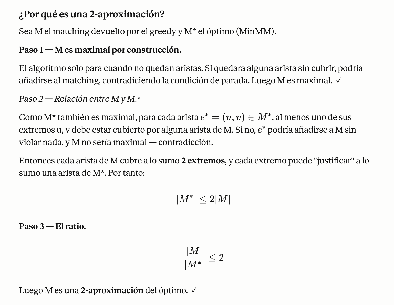
\includegraphics[width=0.8\linewidth]{images/image5.png}
\end{figure}

\href{https://arxiv.org/pdf/1811.08506}{https://arxiv.org/pdf/1811.08506}

\textbf{Connected Cubic graph}
(2518+O(1n))-approximation algorithm for minimum maximal matching in connected cubic graphs.
Que es un connected cubic graph?
Todos los vertices tienen exactamente 3 conexiones, y es conexo.

\href{https://www.combinatorics.org/ojs/index.php/eljc/article/view/v29i2p36/pdf}{https://www.combinatorics.org/ojs/index.php/eljc/article/view/v29i2p36/pdf}
